Following the idea of \textcite{adam.horčík.ea:double}, who used a constrained-optimization example as the utility function of a two-player zero-sum game in \cref{ex.adam21.townsend}, we constructed games based on the dataset of optimization test functions by \textcite{surjanovic13}. Specifically, we selected one example from each shape category: many local minima, bowl-shaped, plate-shaped, valley-shaped, steep ridges, and other.

\strut

\noindent
\begin{minipage}[c]{0.6\textwidth}
\begin{game}\label{ex.adam21.townsend}
A two-player zero-sum game in $1 \times 1$ variables constrained to the intervals
\begin{align*}
x_{11} &\in [-2.25,2.5]\\
x_{21} &\in [-2.5,1.75]
\end{align*}
with the utility given by the \emph{Townsend} function
\begin{align*}
u_1(x_{1}, x_{2}) = x_{11} \sin\left( 3 x_{11} + x_{21} \right) + \cos^{2}\left( \left(x_{11}-0.1 \right) x_{21} \right)
\end{align*}
This game was studied by \textcite[Townsend]{adam.horčík.ea:double}.
\end{game}
\strut
\end{minipage}
\hfill
\begin{minipage}[c]{0.35\textwidth}
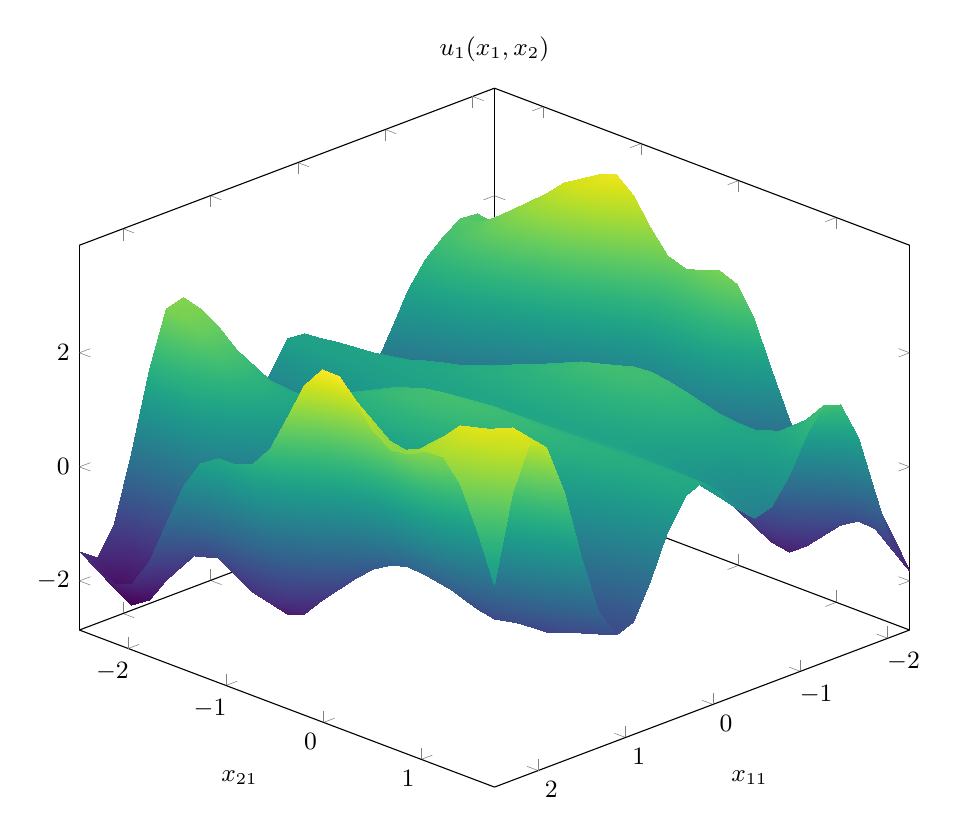
\begin{tikzpicture}
\begin{axis}[
    font=\small,
    domain=-2.25:2.5,
    y domain=-2.5:1.75,
    xlabel=$x_{11}$,
    ylabel=$x_{21}$,
    title={$u_1(x_1,x_2)$},
    colormap/viridis,
    view={135}{30},
    mesh/ordering=y varies,
    width=\textwidth,
]
\addplot3[
    surf,
    shader=interp,
]
{cos(deg((x - 0.1) * y))^2 + x * sin(deg(3 * x + y))};
\end{axis}
\end{tikzpicture}
\end{minipage}



\noindent
\begin{minipage}[c]{0.6\textwidth}
\begin{game}\label{ex.surjanovic.ackley}
A two-player zero-sum game in $1 \times 1$ variables on the interval
\begin{align*}
    x_i &\in [-32.768,32.768] \quad \forall i \in \{1,2\}
\end{align*}
with the utility function \cite[Ackley]{surjanovic13}
\begin{align*}
u_{1}(x_{1}, x_{2}) &=-a e^{-b \sqrt{\frac{1}{2}\sum_{i=1}^2 x_i^2}} - e^{\frac{1}{2}\sum_{i=1}^2\cos(cx_i)} + a + e
\end{align*}
where $a=20$, $b=0.2$, and $c=2\pi$.
\end{game}
\strut
\end{minipage}
\hfill
\begin{minipage}[c]{0.35\textwidth}
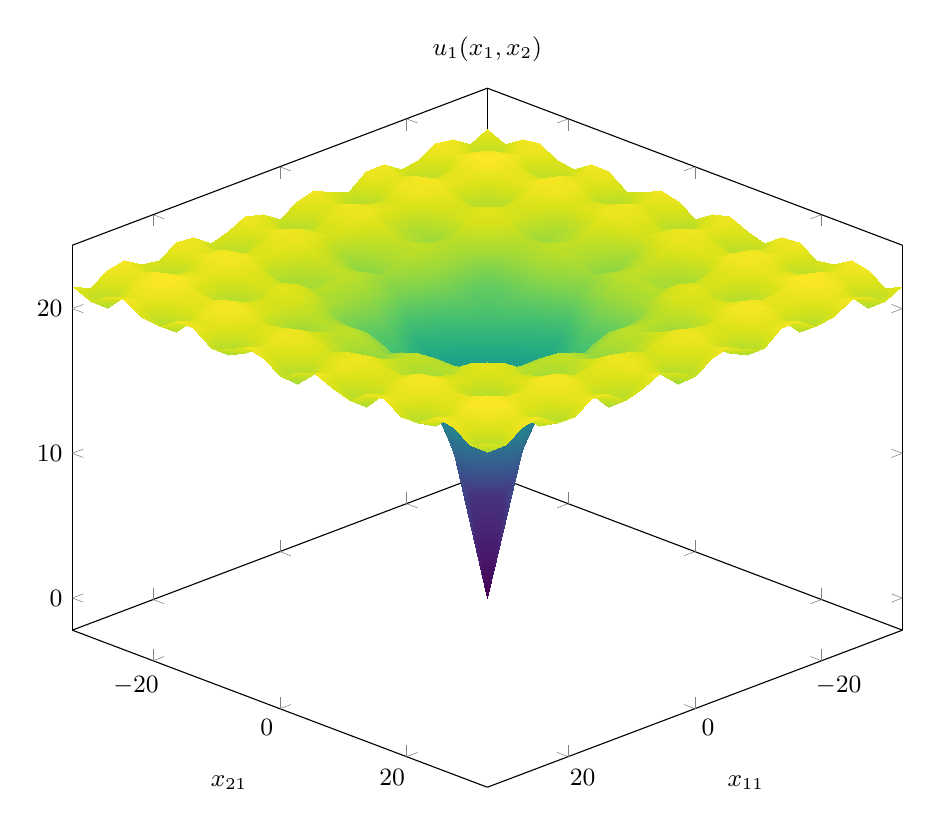
\begin{tikzpicture}
\begin{axis}[
    font=\small,
    domain=-32.768:32.768,
    y domain=-32.768:32.768,
    xlabel=$x_{11}$,
    ylabel=$x_{21}$,
    title={$u_1(x_1,x_2)$},
    colormap/viridis,
    view={135}{30},
    point meta min=5,
    width=\textwidth,
]
\addplot3[
    surf,
    shader=interp,
]
{-20*exp(-0.2 * sqrt((x^2 + y^2)/(2))) - exp((cos(deg(2*pi*x)) + cos(deg(2*pi*y)))/(2)) + 20 + exp(1)};
\end{axis}
\end{tikzpicture}
\end{minipage}




\noindent
\begin{minipage}[c]{0.6\textwidth}
\begin{game}\label{ex.surjanovic.boha1}
A two-player zero-sum game in $1 \times 1$ variables on the interval
\begin{align*}
    x_i &\in [-100,100] \quad \forall i \in \{1,2\}
\end{align*}
with the utility function \cite[Bohachevsky 1]{surjanovic13}
\begin{align*}
u_{1}( x_{1}, x_{2}) &= - 0.3\cos(3\pi x_1) - 0.4\cos(4 \pi x_2) \\ &+  x_1^2 + 2 x_2^2 + 0.7
\end{align*}
\end{game}
\strut
\end{minipage}
\hfill
\begin{minipage}[c]{0.35\textwidth}
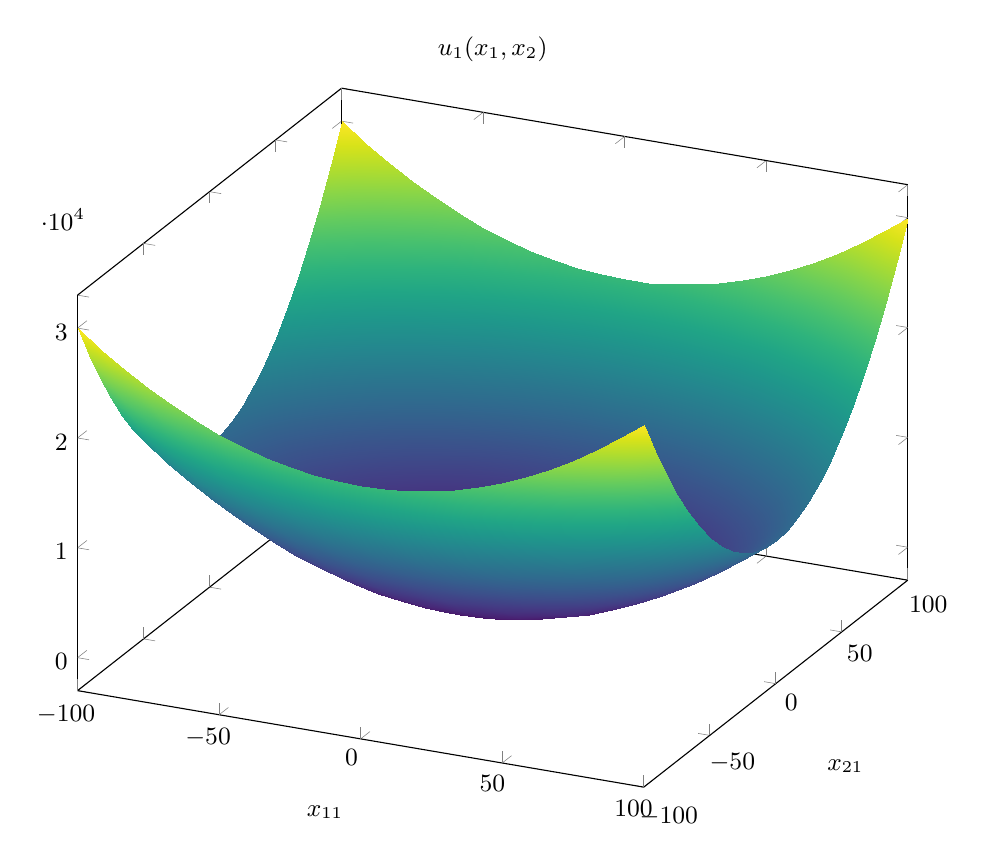
\begin{tikzpicture}
\begin{axis}[
    font=\small,
    domain=-100:100,
    y domain=-100:100,
    xlabel=$x_{11}$,
    ylabel=$x_{21}$,
    title={$u_1(x_1,x_2)$},
    colormap/viridis,
    mesh/ordering=y varies,
    width=\textwidth,
]
\addplot3[
    surf,
    shader=interp,
]
{x^2 + 2 * y^2 - 0.3 * cos(deg(3 * pi * x)) - 0.4 * cos(deg(4 * pi * y)) + 0.7};
\end{axis}
\end{tikzpicture}
\end{minipage}




\noindent
\begin{minipage}[c]{0.6\textwidth}
\begin{game}\label{ex.surjanovic.branin}
A two-player zero-sum game in $1 \times 1$ variables on the intervals
\begin{align*}
    x_1 &\in [-5,10] \\
    x_2 &\in [0,15]
\end{align*}
with the utility function \cite[Branin]{surjanovic13}
\begin{align*}
u_{1}( x_{1}, x_{2} ) &= a (x_2 - b  x_1^2 + c  x_1 - r)^2 \\ &+  s (1 - t) \cos(x_1) + s
\end{align*}
where $a=1$, $b=\frac{5.1}{4 \pi^2}$, $c=\frac{5}{\pi}$, $r=6$, $s=10$, $t=\frac{1}{8\pi}$.

\end{game}
\strut
\end{minipage}
\hfill
\begin{minipage}[c]{0.35\textwidth}
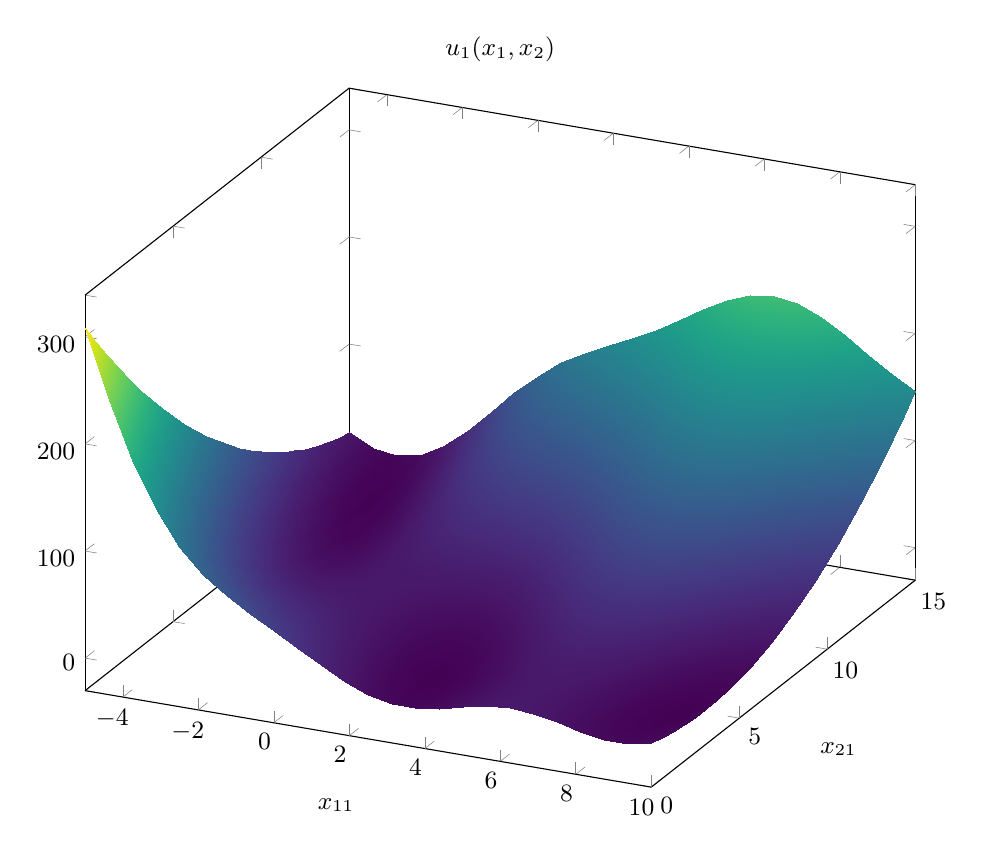
\begin{tikzpicture}
\begin{axis}[
    font=\small,
    domain=-5:10,
    y domain=0:15,
    xlabel=$x_{11}$,
    ylabel=$x_{21}$,
    title={$u_1(x_1,x_2)$},
    colormap/viridis,
    width=\textwidth,
]
\addplot3[
    surf,
    shader=interp,
]
{(y - 5.1 / (4 * pi^2) * x^2 + (5/pi) * x - 6)^2 +  10 * (1 - 1 / (8 * pi)) * cos(deg(x)) + 10};
\end{axis}
\end{tikzpicture}
\end{minipage}




\noindent
\begin{minipage}[c]{0.6\textwidth}
\begin{game}\label{ex.surjanovic.mccorm}
A two-player zero-sum game in $1 \times 1$ variables on the intervals
\begin{align*}
    x_1 &\in [-1.5,4] \\
    x_2 &\in [-3,4]
\end{align*}
with the utility function \cite[McCormick]{surjanovic13}
\begin{align*}
u_{1}{\left( x_{1}, x_{2} \right)} &= \sin(x_1 + x_2) + (x_1 - x_2)^2 - \frac{3x_1 + 5x_2 + 2}{2}
\end{align*}

\end{game}
\strut
\end{minipage}
\hfill
\begin{minipage}[c]{0.35\textwidth}
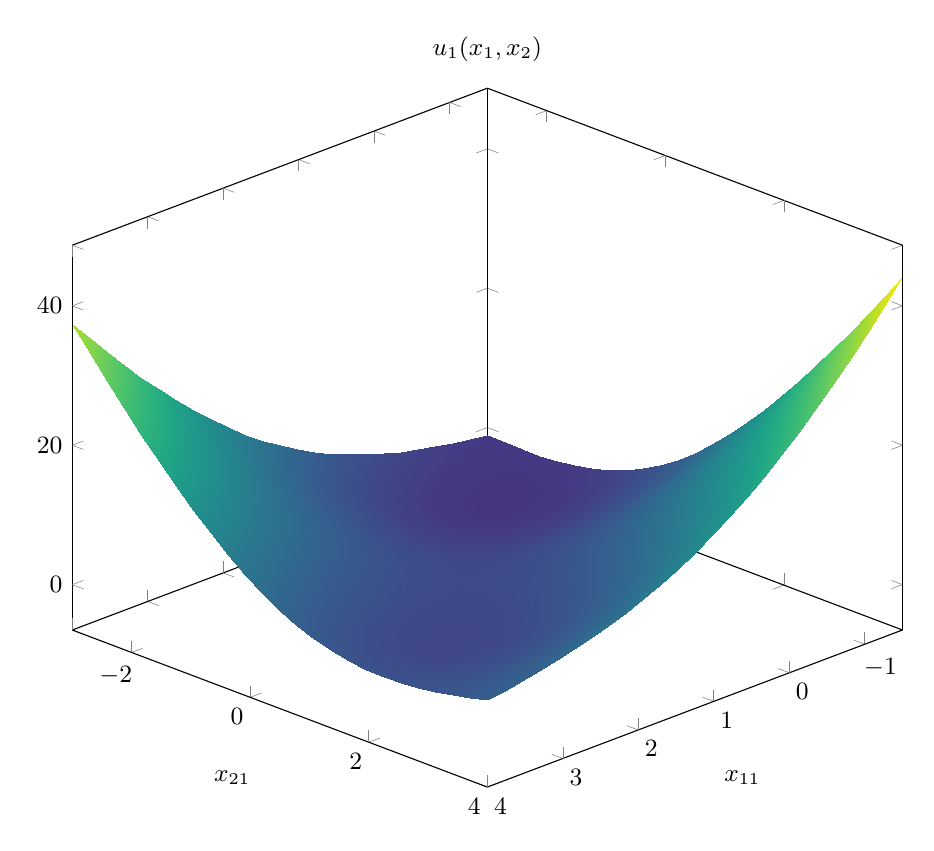
\begin{tikzpicture}
\begin{axis}[
    font=\small,
    domain=-1.5:4,
    y domain=-3:4,
    xlabel=$x_{11}$,
    ylabel=$x_{21}$,
    title={$u_1(x_1,x_2)$},
    colormap/viridis,
    view={135}{30},
    mesh/ordering=y varies,
    point meta min=-10,
    width=\textwidth,
]
\addplot3[
    surf,
    shader=interp,
]
{sin(deg(x + y)) + (x - y)^2 - 1.5*x + 2.5*y + 1};
\end{axis}
\end{tikzpicture}
\end{minipage}



\noindent
\begin{minipage}[c]{0.6\textwidth}
\begin{game}\label{ex.surjanovic.michal}
A two-player zero-sum game in $1 \times 1$ variables on the interval
\begin{align*}
    x_i &\in [0,\pi] \quad \forall i \in \{1,2\}
\end{align*}
with the utility function \cite[Michalewicz]{surjanovic13}
\begin{align*}
u_{1}{\left( x_{1}, x_{2} \right)} &= -\sum_{i=1}^2 \sin(x_i) \sin^{2m}{\left(\frac{i x_i^2}{\pi}\right)}
\end{align*}
where $m=20$.
\end{game}
\strut
\end{minipage}
\hfill
\begin{minipage}[c]{0.35\textwidth}
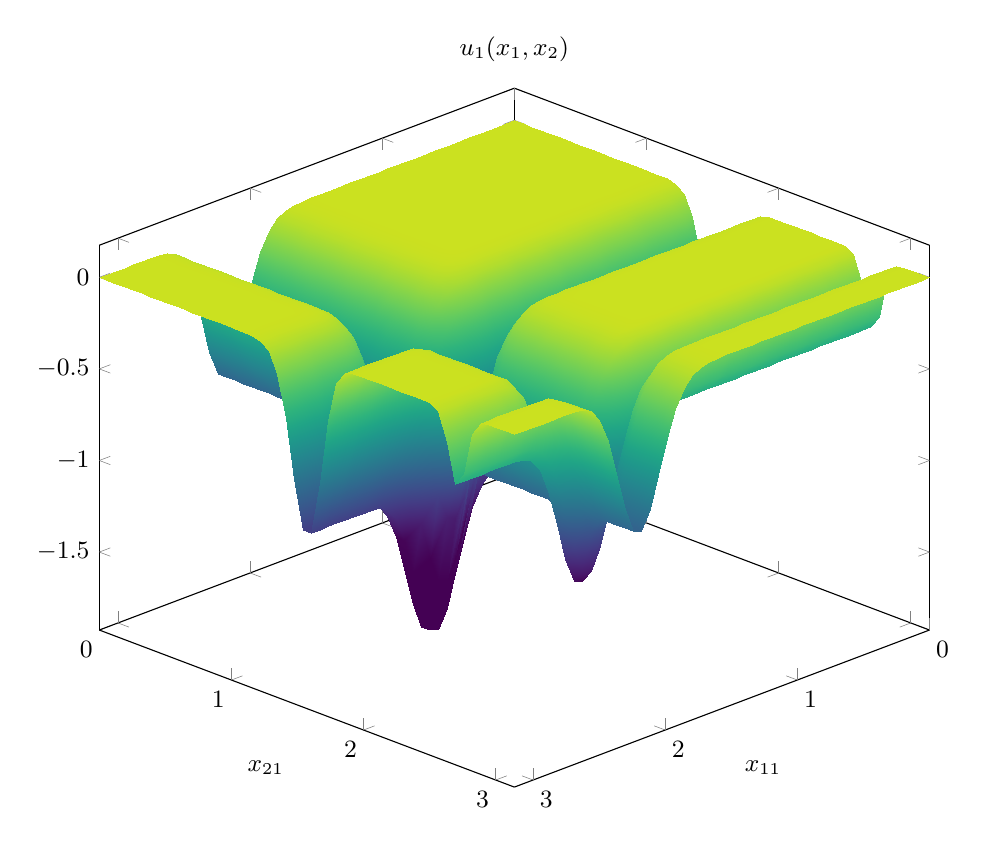
\begin{tikzpicture}
\begin{axis}[
    font=\small,
    domain=0:pi,
    y domain=0:pi,
    samples=50,
    xlabel=$x_{11}$,
    ylabel=$x_{21}$,
    title={$u_1(x_1,x_2)$},
    colormap/viridis,
    view={135}{30},
    mesh/ordering=y varies,
    point meta max=0.1,
    point meta min=-1.2,
    width=\textwidth,
]
\addplot3[
    surf,
    shader=interp,
]
{- sin(deg(x)) * sin(deg(x^2/pi))^20 - sin(deg(y)) * sin(deg(2*y^2/pi))^20};
\end{axis}
\end{tikzpicture}
\end{minipage}



\noindent
\begin{minipage}[c]{0.6\textwidth}
\begin{game}\label{ex.surjanovic.rosen}
A two-player zero-sum game in $1 \times 1$ variables on the interval
\begin{align*}
    x_i &\in [-5,10] \quad \forall i \in \{1,2\}
\end{align*}
with the utility function \cite[Rosenbrock]{surjanovic13}
\begin{align*}
u_{1}{\left( x_{1}, x_{2} \right)} &= 100 (y - x^2)^2 + (x - 1)^2
\end{align*}
\end{game}
\strut
\end{minipage}
\hfill
\begin{minipage}[c]{0.35\textwidth}
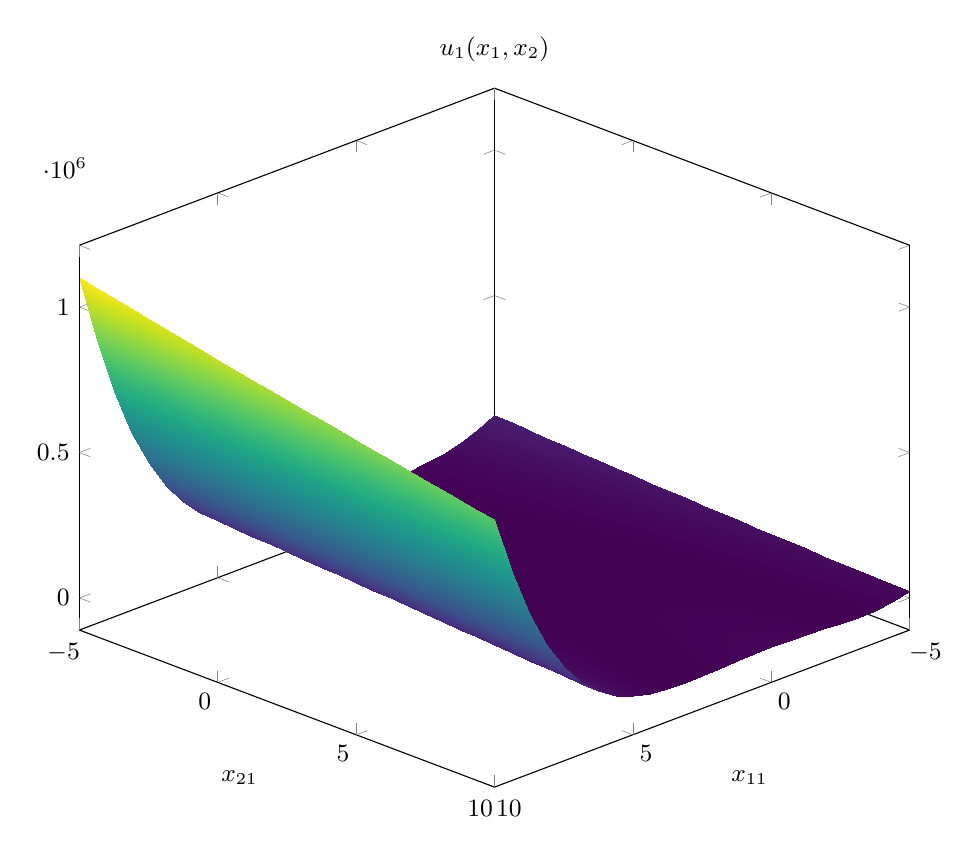
\begin{tikzpicture}
\begin{axis}[
    font=\small,
    domain=-5:10,
    y domain=-5:10,
    xlabel=$x_{11}$,
    ylabel=$x_{21}$,
    title={$u_1(x_1,x_2)$},
    colormap/viridis,
    view={135}{30},
    mesh/ordering=y varies,
    width=\textwidth,
]
\addplot3[
    surf,
    shader=interp,
]
{100*(y - x^2)^2 + (x - 1)^2 };
\end{axis}
\end{tikzpicture}
\end{minipage}